% Este es un documento de LaTeX
\documentclass[12pt]{article}
\usepackage{amsmath,amssymb,graphicx}
\author{Juan David Orjuela}
\date{16 de Agosto de 2015}
\title{Algunos ejemplos con \LaTeX}
\begin{document}
\bibliographystyle{amsplain}
\nocite{Alder1,anderson2008se}
\maketitle
\begin{abstract}
Se presentan unos ejemplos de \LaTeX
\end{abstract}

Aqui va algo de texto, luego empieza una seccion

\section{Ecuaciones}

Un ejemplo de ecuaciones puede ser en linea, como esta $ \vec{F} =m\vec{a} $

\begin{equation}
\vec{F}=m\vec{a}
\end{equation}

\begin{equation*}
\vec{F}=m\vec{a}
\end{equation*}

\section{Tablas}

En la tabla \ref{Ta:Notas}, estan las notas de los parciales
\begin{table}[ht]
\centering
\begin{tabular}{| l | c | r | l |}
\hline
Parcial & 
Primero & 
Segundo & 
Tercero \\ \hline
Ana & 5 & 4 & 3 \\ \hline
Bea & 3 & 4 & 5 \\ \hline
Carlos & 2 & 3 & 4 \\ \hline
\end{tabular}
\caption{Notas de parcial}\label{Ta:Notas}
\end{table}

\section{Figuras}
Esta informacion la tome de \cite{anderson2008}
\begin{figure}
\centering
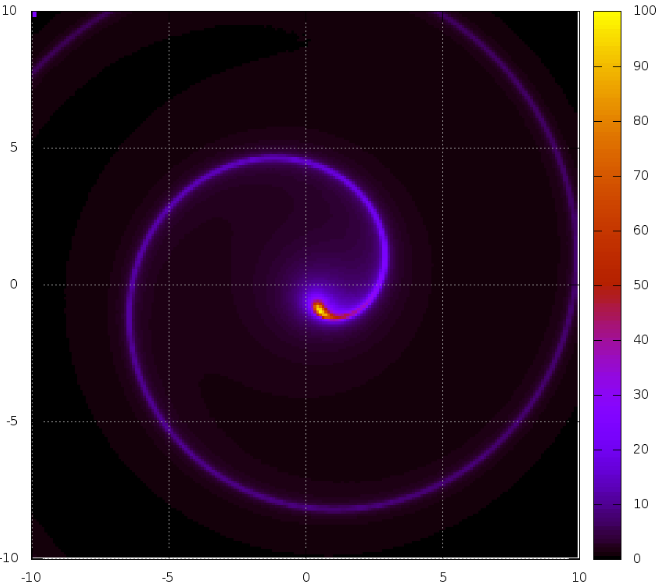
\includegraphics[scale=0.50]{Circulo09c.png}
\caption{Imagen}\label{Fi:Imag}
\end{figure}

%\begin{thebibliography}{9}
%\bibitem{} Frey, G. \textit{Links between stable elliptic curves and certain diophantine equations}, Annales universitatis Saraviensis, \textbf{1} (1986), 1--40. \bibitem{wiles1} Wiles, Andrew, \textit{Modular curves and certain class group}, Invent. Math. \textbf{58} (1980), 1--35. \bibitem{wiles2} Wiles, Andrew, \textit{Modular elliptic curves and Fermat’s Last Theorem}, Annals of Mathematics \textbf{142} (1995), 443--551. \bibitem{taylor-wiles} Taylor, Richard and Wiles, Andrew, \textit{Ring-theoretic properties of certain Hecke algebras}, Annals of Mathematics \textbf{142} (1995), 553--572.
%\end{thebibliography}
\bibliography{biblio}

\end{document}
